\documentclass[25pt,a3paper]{tikzposter}
\usepackage{graphicx}
\usepackage[font=normalsize,labelfont=bf]{caption}
\usepackage{framed}
\usepackage{multirow}
\usepackage[style=nature,maxnames=1,uniquelist=false,backend=bibtex]{biblatex}
\usepackage{hyperref}

% Some field suppression via options
\ExecuteBibliographyOptions{isbn=false,url=false,doi=false,eprint=false}

% One-paragraph bibliography environment
\defbibenvironment{bibliography}
  {\list
     {\printtext[labelnumberwidth]{%
        \printfield{prefixnumber}%
        \printfield{labelnumber}}%
      \ifentrytype{article}{% Suppress remaining fields/names/lists here
        \clearfield{title}}{}}
     {\setlength{\leftmargin}{0pt}%
      \setlength{\topsep}{0pt}}%
      \renewcommand*{\makelabel}[1]{##1}}
  {\endlist}
  {\mkbibitem}

% \mkbibitem just prints item label and non-breakable space
\makeatletter
\newcommand{\mkbibitem}{\@itemlabel\addnbspace}
\makeatother

% Add breakable space between bibliography items
\renewcommand*{\finentrypunct}{\addperiod\space}

% et al. string upright (nature style applies \mkbibemph)
\renewbibmacro*{name:andothers}{%
  \ifboolexpr{
    test {\ifnumequal{\value{listcount}}{\value{liststop}}}
    and
    test \ifmorenames
  }
    {\ifnumgreater{\value{liststop}}{1}{\finalandcomma}{}%
     \andothersdelim
     \bibstring{andothers}}
    {}}

\addbibresource{../refs}
  
\graphicspath{/home/james/Documents/University/3/Project/FullUnit_1819_JamesKing/ProjectReports/DemoPoster/}
\definecolor{mygray}{HTML}{CCCCCC}
\definecolorstyle{myColorStyle}{
}{% Background Colors
	\colorlet{backgroundcolor}{black!50}
	\colorlet{framecolor}{black!50}
	% Title Colors
 	\colorlet{titlefgcolor}{white}
 	\colorlet{titlebgcolor}{black}
 	% Block Colors
 	\colorlet{blocktitlebgcolor}{black}
 	\colorlet{blocktitlefgcolor}{white}
 	\colorlet{blockbodybgcolor}{mygray!50}
 	\colorlet{blockbodyfgcolor}{black}
 	% Innerblock Colors
 	\colorlet{innerblocktitlebgcolor}{black}
 	\colorlet{innerblocktitlefgcolor}{white}
 	\colorlet{innerblockbodybgcolor}{white}
 	\colorlet{innerblockbodyfgcolor}{black}
 	% Note colors
 	\colorlet{notefgcolor}{black}
	\colorlet{notebgcolor}{white}
	\colorlet{notefrcolor}{white}
}
\usebackgroundstyle{Rays}
\useblockstyle{Slide}
\usetitlestyle{Wave}
\usecolorstyle{myColorStyle}
\usepackage{multicol}

\begin{document}
\title{Cooperative Strategies in Multi-Agent Systems}
\author{James King}
\maketitle
\begin{columns}
\column{.5}
\block{Aim}{
	To study how game-theoretic techniques can be leveraged in MASs to create cooperative societies of agents.
}
\block{Objectives}{
	\begin{itemize}
		\item Develop a theoretical framework for a MAS where agents interact using game-theoretic techniques
		\item Implement this framework in a distributable architecture
		\item Run experiments using the implementation
		\item Analyse the experiments and evaluate the results to understand the effectiveness of the techniques used in the theoretical framework
	\end{itemize}
}
\block{The Nature Engine}{
	The web application
}
\block{The Environment}{
	\begin{minipage}{16cm}
		\begin{framed}
		\begin{center}
			\begin{tabular}{c|c|c}
			\multirow{2}{*}{Donor Action} & \multicolumn{2}{c}{Payoffs}\\	
			& Donor & Recipient\\
			\hline
			Cooperation & -1 & 2\\
			\hline
			Defection & 0 & 0\\
			\end{tabular}
			\captionof{table}{The payoff for Nowak and Sigmund's~\parencite{evolution_of_cooperation} indirect reciprocity model}
			\label{tab:indirrec_payoffmatrix}
		\end{center}	
		\end{framed}
	\end{minipage}
	\begin{minipage}{22cm}
		The environment that my agents reside in cycles through a user chosen number of timepoints in which the agents receive percepts from the environment, revise their beliefs according to their trust model and then decide on an action according to their strategy. These steps are synchronised so that agents act simultaneously without knowledge of other actions at that timepoint.\\
	\end{minipage}
	At each timepoint a donor-recipient pair is randomly selected from the population, as well as a set of onlookers. The donor at this timepoint is limited to either cooperating or defecting. Each player has a fitness score which represents their success in the society. Being part of a donor-recipient pair is the only way in which  this fitness is affected, the effects on fitness are shown in the payoff matrix above.\\\\
	The onlookers and recipient receive a percept in the next timepoint of the action that has been committed to by the donor. All other agents at that timepoint are able to commit to gossip or idle actions. Gossip actions generate a percept which is perceived by the recipient of the gossip in the next timepoint. This gossip is either positive or negative about a subject agent.
}
\block{Genetic Algorithm}{
	From each simulation we wish to find the most successful strategies out of a set of strategies. This is a type of optimisation problem. We can emulate the process of evolution to tackle optimisation problems using genetic algorithms.\\\\
	A genetic algorithm runs through a number of generations. Each generation is an instance of the environment with a unique set of agents. Between each generation agents are reproduced proportionately to their fitness using a reproduction step algorithm - 	roulette wheel selection via stochastic acceptance~\parencite{lipowski2012roulette} which runs in $O(n)$ run-time for n agents. 
}
\block{Agent Strategies and Trust Models}{
	
}
\column{.5}
\block{Agents}{
	\begin{minipage}{18cm}
		There are many conflicting views of what an agent truly is. Most agree that it is a computer program or system that adheres to a few properties or a programming paradigm. Wooldridge and Jennings~\parencite{wooldridge_jennings_1995} stipulated 4 properties that qualifies the system as an agent:
		\begin{itemize}
			\item Autonomy
			\item Social Ability
			\item Reactivity
			\item Pro-activeness
		\end{itemize}
		Agents reside within an environment. Russell and Norvig define an agent as anything the perceives and acts on it's environment. 
	\end{minipage}
	\begin{minipage}{3cm}
	\end{minipage}
	\begin{minipage}{18cm}
		\begin{framed}
			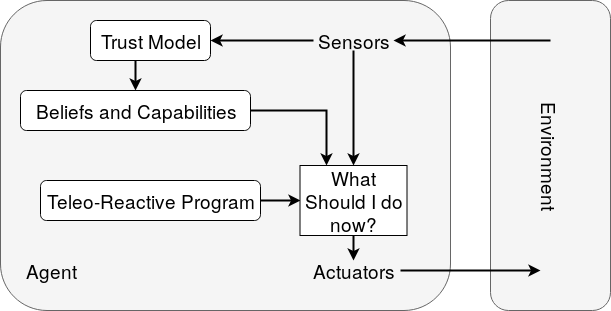
\includegraphics[width=\textwidth]{AgentArchitecture.png}
			\captionof{figure}{Agent architecture}
		\end{framed}
		Agents are typically built with an architecture which defines the components that make up the inner workings of the agent. Many of these architectures make use of concepts from the beliefs-desires-intentions model~\parencite{bratman1987intention}, including the architecture for this project's agents which is illustrated above. 
	\end{minipage}
}
\block{Multi-Agent Systems and Agent Interactions}{
	\begin{minipage}{22cm}
		\begin{framed}
			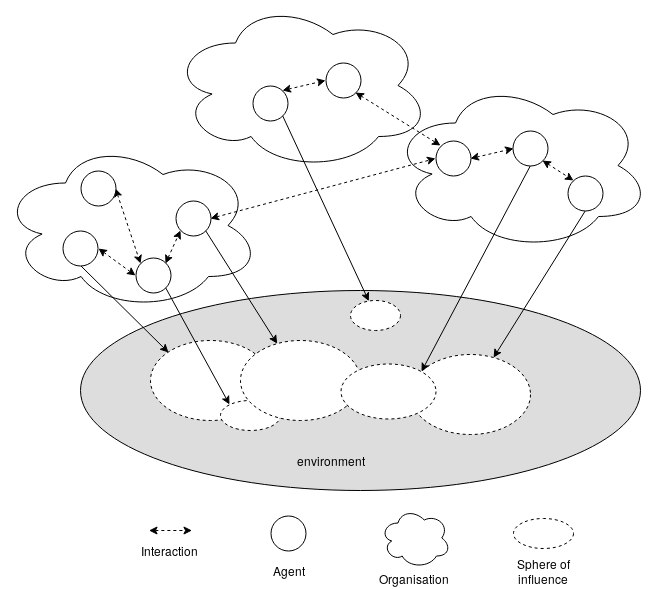
\includegraphics[width=\textwidth]{JenningsMAS.png}
			\captionof{figure}{Jennings'~\parencite{jennings2000agent} depiction of a multi-agent system}
		\end{framed}
	\end{minipage}
	\begin{minipage}{16cm}
		A multi-agent system is a group of agents that are situated in the same environment and are capable of interacting with each other. Interactions occur through agents committing to actions including speech acts. Agent communication languages (ACLs) facilitate speech acts. In my system agents interact through donor actions and speech acts using the Simple Agent Gossip Language (SAGL).\\\\
		When agents interact they decide on actions according to a strategy which describes how an agent should act in any circumstance it finds itself in. These strategies attempt to account for other agents' decisions and maximise the agent's utility.
	\end{minipage}
}
\block{Reciprocal Altruism}{
	\begin{minipage}{12cm}
			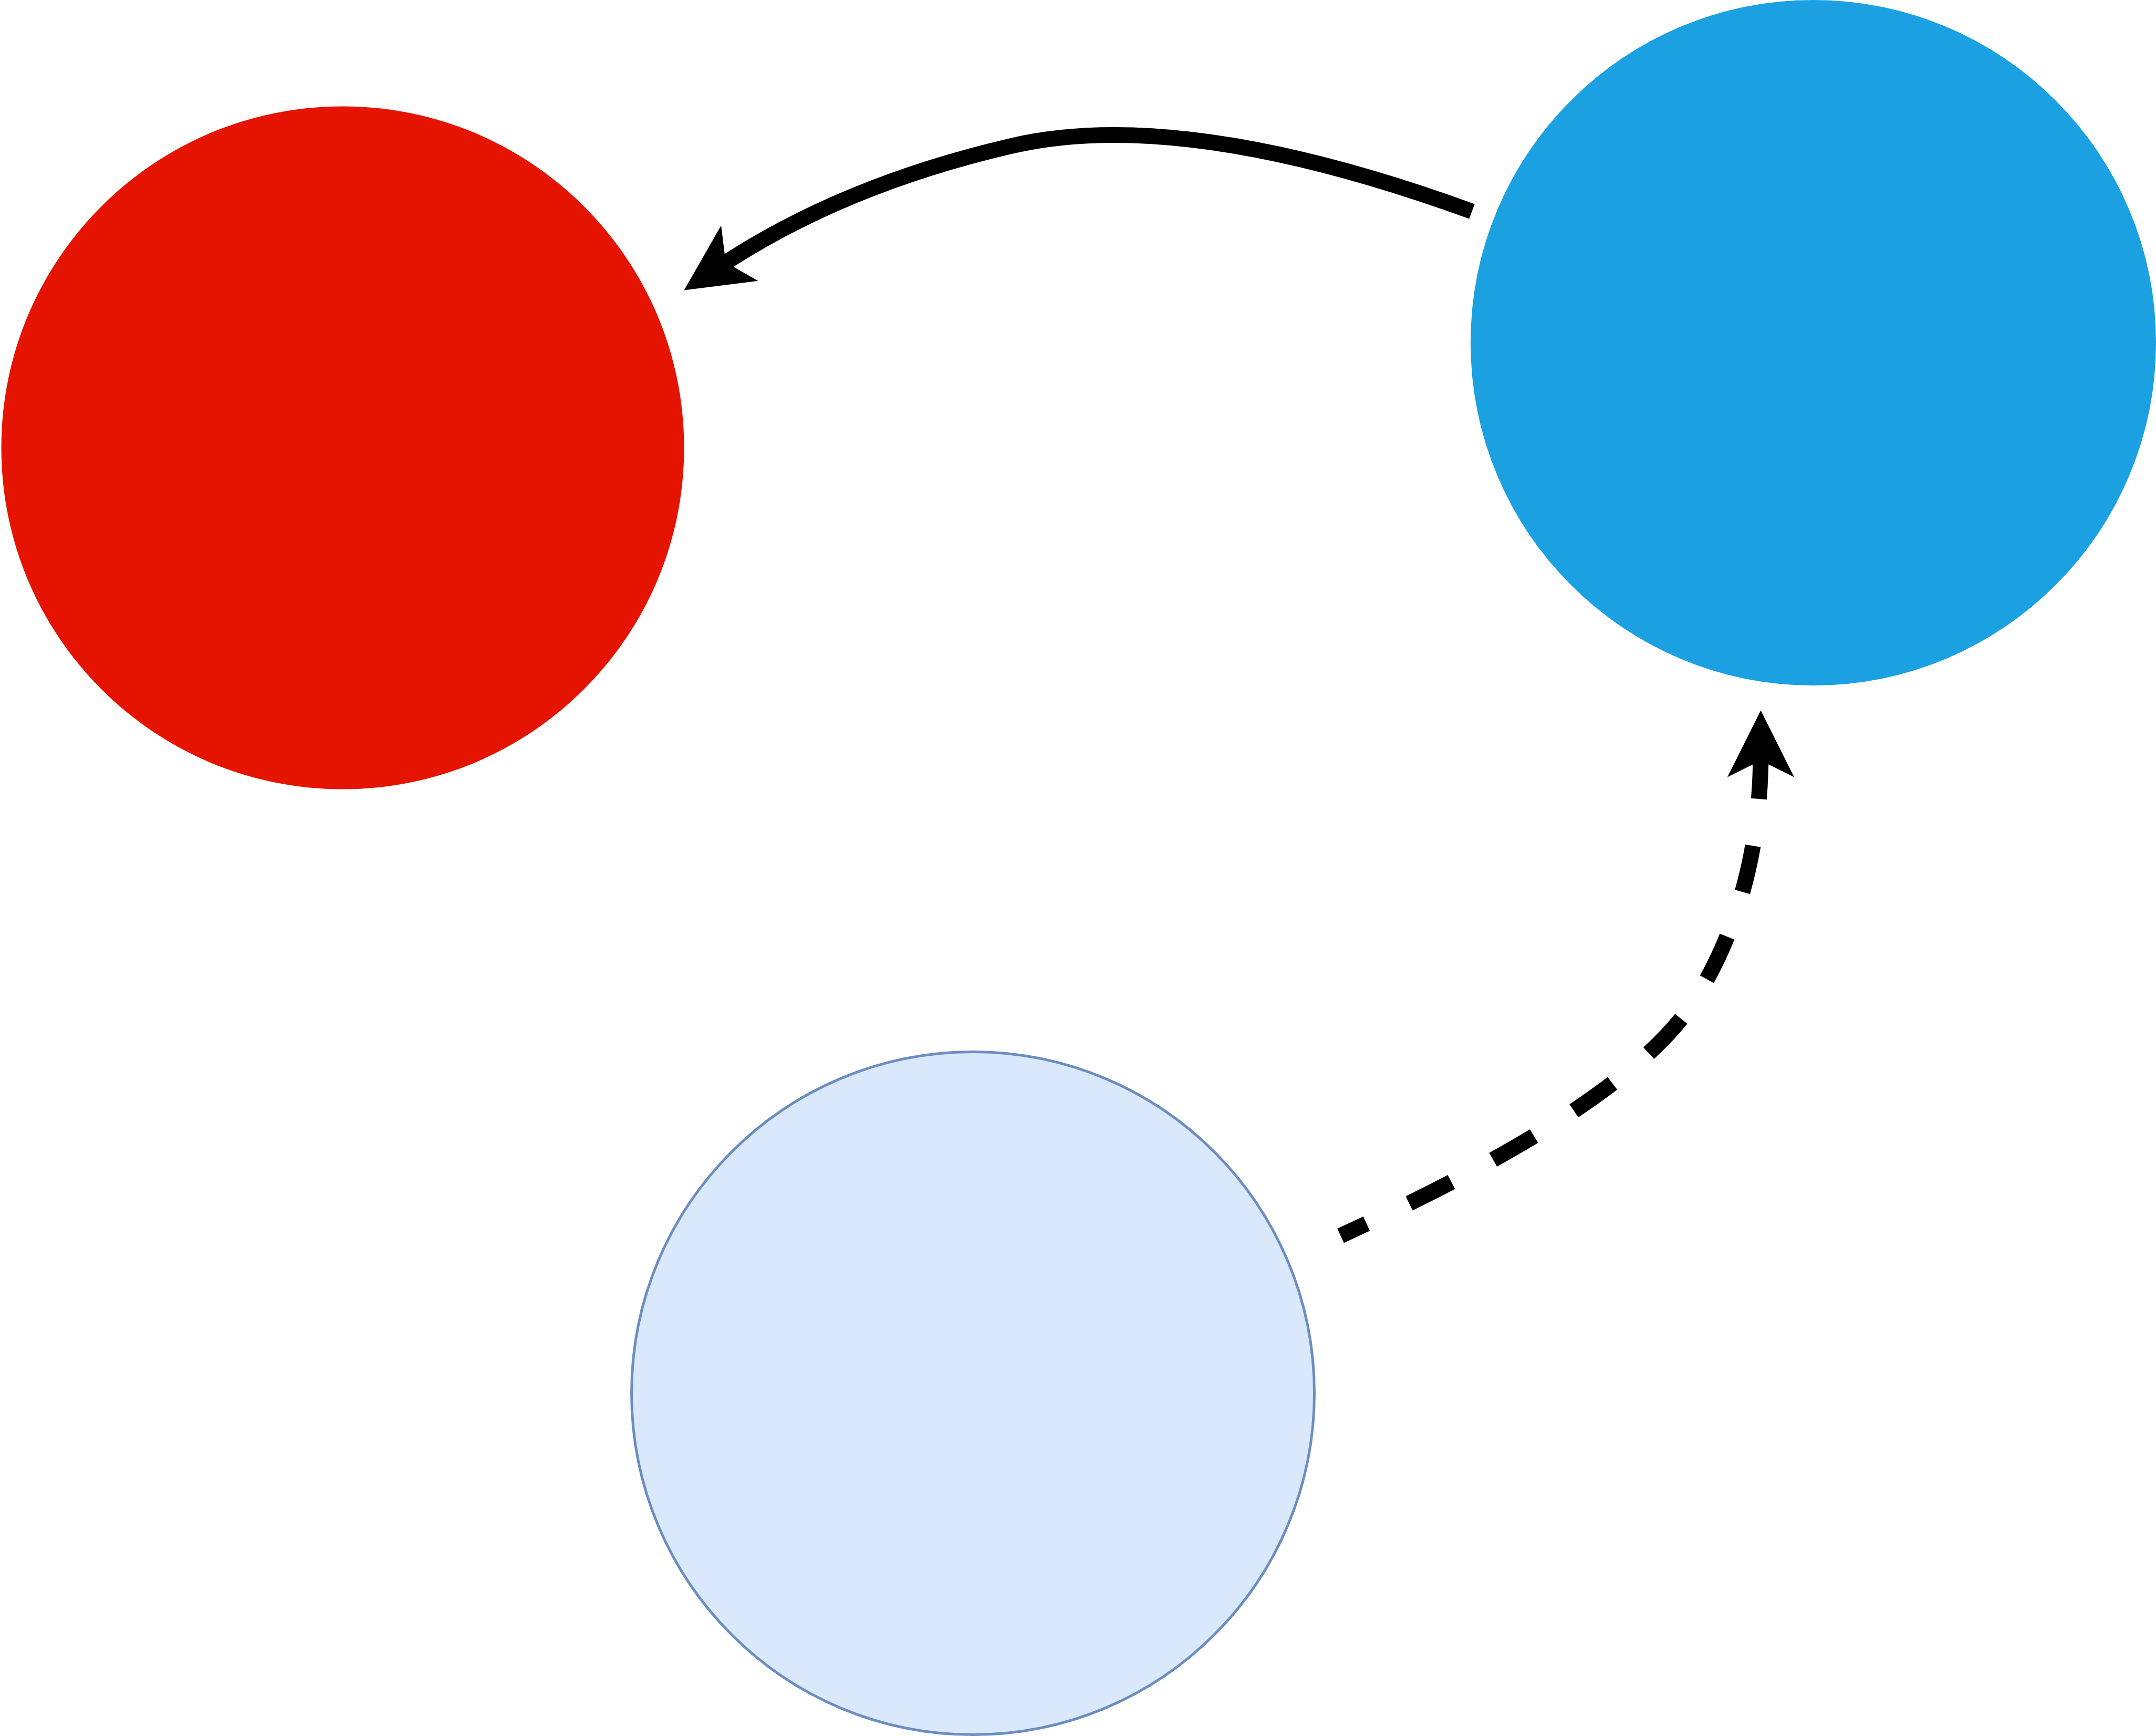
\includegraphics[width=\textwidth]{IndirectRec.png}
			\captionof{figure}{Indirect reciprocity is a mechanism where agents act altruistically expecting third parties to reciprocate the act}
	\end{minipage}
	\begin{minipage}{12cm}
		
\includegraphics[width=\textwidth]{DirectRec.png}
		\captionof{figure}{Direct reciprocity is a mechanism where agents act altruistically expecting the receiving party to reciprocate the act}
	\end{minipage}
	\begin{minipage}{12cm}
		Reciprocal altruism~\parencite{trivers1971evolution} is a concept in evolutionary biology which attempts to explain the evolution of cooperation. The idea is that agents commit to actions that are temporarily detrimental to them and beneficial to others with the expectation that their altruism will be remunerated by others.\\
	\end{minipage}
		Game theory has taken up this idea in modelling the evolution of cooperation in many forms - most importantly for us direct reciprocity~\parencite{evolution_of_cooperation} and indirect reciprocity~\parencite{evol_indirect_image} illustrated to the left. These ideas can be leveraged in the design of multi-agent systems to produce cooperative societies of agents.
}
\block{Citations}{
 	\begingroup
	\renewcommand{\section}[2]{}
	\printbibliography
	\endgroup
}
\end{columns}
\end{document}
